\documentclass[11pt]{article}
\usepackage[margin = 1in]{geometry}
\usepackage[utf8]{inputenc}
\usepackage{pdfpages}
\usepackage{cite}
\usepackage{amsmath,amssymb,amsfonts}
\usepackage{algorithmic}
\usepackage{graphicx}
\usepackage{textcomp}
\usepackage{xcolor}
\usepackage{url}
\usepackage{subfig}
\usepackage{bm}
\usepackage{caption}
\usepackage{multirow}
\usepackage{dirtytalk}
% \usepackage{subcaption}
\usepackage{lipsum}
\usepackage{tikz,graphics,color,float,epsf,caption}

% \usepackage[
%     backend=biber,
%     citestyle=numeric,
%     style=numeric,
%     sorting=none]{biblatex}
    
\usepackage{titlesec}
\usepackage[font=scriptsize]{caption}
\usepackage{wrapfig}
% \usepackage{subcaption}
\usepackage{fancyhdr}

% Example definitions.
% --------------------
\def\x{{\mathbf x}}
\def\L{{\cal L}}

\DeclareMathOperator*{\argmin}{argmin}
\DeclareMathOperator*{\Proj}{Proj}

\graphicspath{ {./Figures/} }

% loading subfig class according to IEEE
% \ifCLASSOPTIONcompsoc
% \usepackage[caption=false,font=normalsize,labelfont=sf,textfont=sf]{subfig}
% \else
% \usepackage[caption=false,font=footnotesize]{subfig}

\pagestyle{fancy}
\renewcommand{\headrulewidth}{0.2pt}
\fancyhead[L]{Kaveen Liyanage}
\fancyhead[R]{SR based FR methods}

\begin{document}
\input{titlepage}


\input{summary}

\newpage
% \rfoot{\small\thepage}
\section{Introduction}
With the rise of information collection by different methods and agencies, the amount of data to consider before making decisions has become a significant challenge. Some examples of data collected in a medical environment are age, gender, weight, blood pressure, etc. These types of data collected are considered as features or dimensions in the final dataset. Often these features are unnecessary, redundant, or highly co-related to the application at hand. Further, they do not provide any new information about the subject matter to make a good decision. When these large collections of data are used in machine learning (ML) models, they consume more time, energy, and resources and produce sub-par results. The idea of \say{Garbage in, Garbage out} is in effect for most ML models. This means, that unnecessary information sometimes directs the ML models to learn wrong patterns, which leads to useless models.  Especially with the ML concept of \textit{black box} models, it is even harder to identify the significant features and the redundant features which contribute to the final decisions.

\subsection{Feature Ranking}

Because of this, Feature Ranking (FR) is an essential part of the machine learning pipeline to identify, reduce, remove, or craft features that benefits ML performance and reduce the cost of the operations. FR methods evaluate the features by looking at the amount of information they provide and rank them accordingly. So, the most relevant and complementary features would have higher scores and can use in ML training. There are three main categories of methods for FR algorithms, which are Filter methods (FM), Wrapper methods (WM), and Embedded methods (EM). FR methods are further classified as {\it myopic} and {\it non-myopic}. Where {\it myopic} methods only evaluate the feature by itself, while {\it non-myopic} methods take into consideration the inter-relationships between the features.

There are few surveys done to understand the pros and cons of the current state of the art in feature assessment techniques \cite{Uthman2020, Sangodiah2014, Effrosynidis2021, Jovic2015}. A summary of the method's pros and cons are shown in fig.\ref{fig: FR_methods}. In FM, intrinsic properties are evaluated like entropy, variance, and auto-correlation to determine the relevance of the feature. FM methods are generally computationally inexpensive and do not depend on the ML model as the evaluation is done independently. In WM the feature ranking is tied to the ML model performance. Every feature that contributes to the improvement of the ML model is given a higher ranking. This method is more computationally expensive than the FM as it needs to train multiple ML models to identify which features contribute more. WM is model and tasks specific hence, giving better results. However, WM FR has to be performed again for a different task or a model. EM is similar to WM, however, it performs the feature selection while the ML model is training. Therefore, time can be saved by avoiding training just a single model. However, performance is sacrificed compared to WM. EM is also model and task-specific. 

\begin{figure}[!t]
    \centering
    \includegraphics[width=12cm]{Figures/FR_methods.png}
     \caption{Classification of the FR methods and summary of pros and cons}
    \label{fig: FR_methods}
\end{figure}


\subsection{Problem}
Although many FR algorithms exist, there is no universal method. Each FR method focuses on different aspects of the features depending on applications requirements. The problems identified in common FR metrics and aiming to address are as follows.

\begin{enumerate}
    \item Interpretability.
    
    Some of these measures are highly non-linear and complex, it is hard to have an intuitive understanding of the FR process. There is no direct/linear relationship between the features and the ML model behavior.
    
    \item Class-wise feature relevance.
    
    Most of the FR methods cannot determine class-wise FR in the presence of multiple classes. Especially in FM, although FR can be applied to each class separately or as a whole, they cannot distinguish feature relevance for each class. The relationship between the classes is not considered when ranking is calculated for a single class.
    
    \item Imbalance class data.
    
    Some traditional FR methods do not consider the class distributions or the class imbalances. This affects unfavorably small classes of the dataset as the larger classes will overwhelm the FR metric. This becomes a significant problem when you are trying to detect abnormalities/ outliers or have small sample size classes. For example, in a medical computational topology(CT) scan you might have rare occurrences of lesions. If you just apply FR metrics to find the best features to represent the CT images it will find the \say{best} of features to represent the majority of the images. Which could omit features that would be specific to represent the small number of lesions.  
\end{enumerate}

\subsection{A Solution}

Sparse representation (SR) is a method of increasing the dimensions of the dataset to achieve a better representation of the data \cite{Elad2010}. This process is linear and easier to understand. In SR, the process is divided into two steps. First, it learns a dictionary of subspaces of original feature space. These, subspaces or the dictionary elements are \say{atoms}. Second, it tries to approximately represent each datum as a linear combination of those dictionary atoms. In practice, these two processes are iteratively optimizing each other until a stopping criterion is met. SR methods are effective in several under several assumptions. One is the original data is laying in a subspace of the original feature space This assumption seems to be true for applications like images and music analysis. The learned atoms reveal some information about the data distribution in the original feature space. 

Hence, we are proposing a method that will use SR to identify important features for FR tasks. The \textit{dictionary mapping}, and \textit{dictionary utilization} are introduced as novel and simple metrics for FR tasks. These metrics evaluate the learned dictionary atoms and linearly transform them to the original feature space. This allows us to observe the atom distribution in the original feature space. These methods are \textit{non-myopic} and a hybrid of FM and EM concepts. To calculate the metrics, dictionary learning has to be carried out (like EM), which is more computationally expensive than the typical FM. However, these metrics do not depend on any ML methods. Unlike, EM methods these FR scores can be used in many applications. Furthermore, the proposed metrics do not depend on any particular dictionary learning method. However, using a discriminatory dictionary learning and (semi-)supervised SR method would be able to improve the interpretation ability of the data. Since the atoms are a subspace of the original feature space when atoms are learned it takes into account the relationship between all the features hence, these metrics are \textit{non-myopic}. Figure \ref{fig: SR_sol} summarizes the issues identified and the aspects of the SR that would help improve/address each of the issues pertaining to common FR metrics. It should be noted that not every FR metric has these issues, and might address one or more issues. However, with SR methods we could improve all of the issues at once.

\begin{figure}[!t]
    \centering
    \includegraphics[width=12cm]{Figures/SR_sol.png}
    \caption{Issues with common FR methods, the common causes and the properties of SR which could improve the issues}
    \label{fig: SR_sol}
\end{figure}

Preliminary tests with sample datasets show that these metrics perform similarly to some selected FR methods as shown in fig.\ref{fig: FR_degradation}. Class-wise representation of the FR metric was useful in identifying relevant features for each class. Which cannot be generated using the selected FR methods. Furthermore, the learned sparse representation of the data as a by-product of learning the dictionary is not wasted. Those SR coefficients can be used to train ML models. If the original data is sparse, it is shown that using a simpler (linear) ML model using SR would be sufficient to achieve on-par results. However, in practice, these ML performances are slightly sub-par to the performances of ML models trained with original features. There is a trade-off between explainable simpler ML models and high-performing complex ML models. We would argue with the added benefit of the FR capabilities even sub-par performing simpler ML models will be the better option for certain applications. Especially in the developing stage where you want to identify and analyze model and feature behavior.

\begin{figure}[!t]
    \centering
    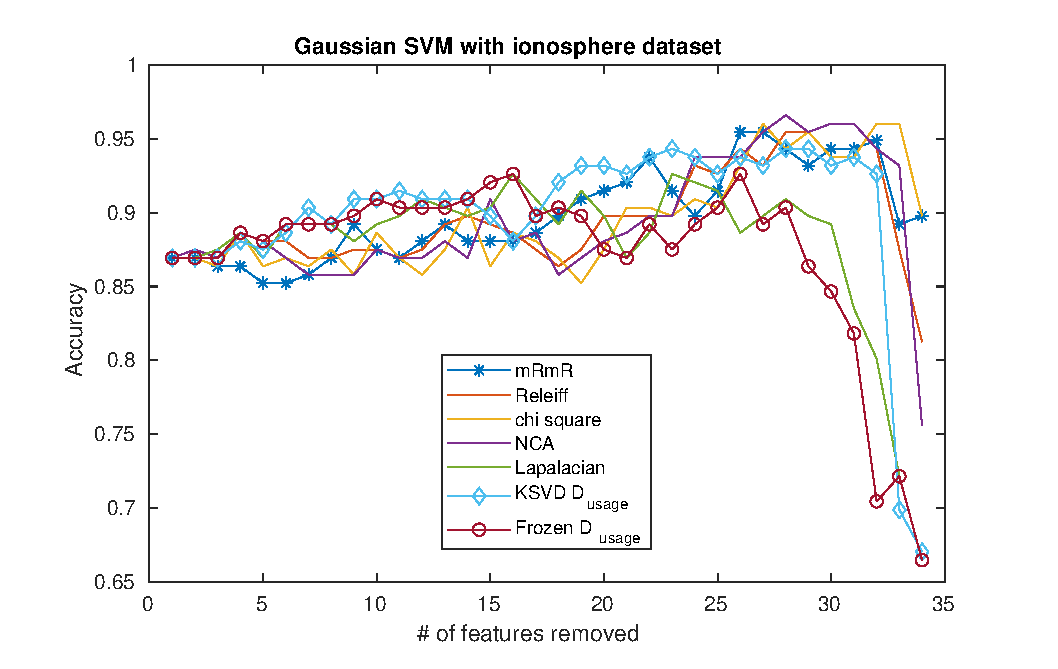
\includegraphics[width=12cm]{ion_gauss.eps}
    \caption{Classifier performance degradation with number of features removed. It can be observed that the proposed methods have less performance degradation than the common FR metrics.}
    \label{fig: FR_degradation}
\end{figure}

In this proposal, we are planning to show the robustness and the versatility of the proposed FR metrics. We will test the proposed FR metrics on several common datasets as well as synthetic datasets while comparing them to other common FR methods. This will allow us to perform necessary improvements on the metrics. With discriminatory SR methods, we will perform tests to identify the methods that have the best interpretation ability. Finally, the FR metrics are to evaluate two real-life problems. Namely, satellite image classification and Malware detection. We hope that the proposed metric will help future researchers in identifying and analyzing features effectively without wasting time and effort using unnecessary features.

\section{Background}

\subsection{Sparse Representation and Dictionary Learning}

Let $\mathbf{F} = [F_1, F_2, \dots F_d]$ be a set of $d$ features $F$ which are collected or curated. The goal is to rank the feature set $\mathbf{F}$ by evaluating a mean-removed training set of $n$ samples: $\mathbf{\bar{Y}} = [y_1, y_2, \dots, y_n] \in \mathbb{R}^{d \times n}$. The set of $k$ classes is defined as $\mathbf{C} = [C_1, C_2, \dots, C_k],$ where each of the $x$ samples is assigned to a class $C$. In sparse representation the input sample is represented as a linear combination of dictionary elements $D$ in a over-complete ($d \ll m$) dictionary $\mathbf{D} = [D_1, D_2, \dots, D_m] \in \mathbb{R}^{d \times m}$, where the number of dictionary elements used, $s$, is far less than the number of dictionary atoms: $s \ll m$. The set coefficients $\bm{\alpha} = [\alpha_1, \alpha_2, \dots, \alpha_n] \in \mathbb{R}^{m \times n}$ of the linear combination is called the sparse coefficients. Each coefficient vector contains $s$ nonzero entries; the remaining $m-s$ entries are exactly zero. The general objective function used for calculating the sparse representation is given by (\ref{eq:sparse}) with an $\ell_0$ constraint on sparsity.

\begin{equation}
    \label{eq:sparse}
    \argmin_{\mathbf{D},\bm{\alpha}} ||\mathbf{\bar{X}}- \mathbf{D}\bm{\alpha}||_F + ||\bm{\alpha}||_0
\end{equation}

The KSVD algorithm is an efficient iterative method that solves the objective function by, first fixing the $\mathbf{D}$ and optimizing the $\bm{\alpha}$ using orthogonal matching pursuit (OMP)\cite{Pati1993}. Second, it fixes $\bm{\alpha}$ then optimize $\mathbf{D}$ with generalized K-means and singular value decomposition (SVD). Figure \ref{fig: DictLearn} represent the input signal, learned dictionary, and the sparse coding as a matrix. Since the learned dictionary is over-complete, the spread of the dictionary atoms can give an insight into which features are more relevant for the representation. Hence, we will be defining simple metrics that will quantify the spread of the dictionary elements in each of the features. 

\begin{figure}
    \centering
    \includegraphics[width = 0.4\textwidth]{Figures/DictLearn.JPG}
    \caption{Matrix representation of the input signal, learned dictionary, and the sparse coefficients}
    \label{fig: DictLearn}
\end{figure}

In LC-KSVD \cite{Jiang2011}, the algorithm employs an objective function comprised of reconstructive, discriminative, and classification costs. The LC-KSVD dictionary is initiated by equally dividing among the classes. Then class labels are used to force the dictionary atom learning to be constrained into the predefined dictionary locations. However, this method does not takes into account class imbalances.

Frozen dictionary learning is a modification of traditional sparse coding dictionary learning that attempts to learn a dictionary that can effectively model imbalanced datasets\cite{Carroll2017}. In this algorithm first, the dictionary learning step is carried out using an algorithm, then the learned dictionary elements are held constant and the dictionary is augmented with additional elements. For the next step, the dictionary is trained again on data containing abnormalities. The frozen elements of the dictionary represent the normal aspects of the data, hence the new elements (non-frozen) learn to represent the anomalous aspects of the data that are not present in the normal data. The frozen dictionary approach could be generally used and applied to the problems including data with or without abnormalities. 

\begin{figure}
\begin{centering}
    \subfloat[][]{\includegraphics[width=.4\textwidth]{Input domain.JPG}
    \label{fig:Indomain}}
    \qquad
    \subfloat[][]{\includegraphics[width=.4\textwidth]{Dict domain.JPG} 
    \label{fig:Dictdomain}}
    % \subsection{Dictionary atoms domain}
    
    \caption{(a) Sparse representation of the input data with dictionary atoms. (b) Classifier in the dictionary atoms domain.}
    \label{fig:image2}
\end{centering}
\end{figure}


Figure \ref{fig:Indomain} illustrates the representation of the input signals with the learned dictionary atoms in a two-dimensional input feature domain with sparsity, $S =2$. $y_1, y_2$ are the input signals belonging to two separate classes. With LC-KSVD the algorithm forces dictionary atoms $d_1, \dots , d_3$ to be used for $y_1$ in class 1 and $d_4, \dots , d_6$ to be used for $y_2$ in class 2. Fig. \ref{fig:Dictdomain} illustrates the learned classifier boundary in the (sparse) domain of $d_1$ and $d_4$. Due to the class constraints in the dictionary learning process, the majority of the input data will only be represented by the dictionary atoms corresponding to their class. Thus in the sparse domain, most signals will lie in a class-specific subspace of the entire dictionary. Hence, a linear classifier can be utilized for the classification with satisfactory results. Further, there is a direct relationship between the classifier domain and the input domain. 

\section{Goals}

\begin{enumerate}
    \item \textbf{Improve the interpretability of the Feature selection criteria}.
    
    Existing FR methods show a lack of class-wise interpretability. Through this proposal, we will try to improve the interpretability of FR by employing two FR metrics based on SR. We will exploit the simplicity and the linearity of the SR methods to improve interpretability.
    
    \item \textbf{Addition of feature ranking as a functional advantage of sparse representation}
    
    SR has many proven applications in the image reconstruction domain. With this proposal, we are hoping to add new functionality to SR as an FR technique.  
    \item \textbf{Exploration of SR usage as a  sparse graph kernel in computer-security domain}
    
    Application of the SR methods in the computer security domain is rare. We will develop a framework to apply SR as a sparse graph kernel to detect malware using control flow diagrams of the programs.
\end{enumerate}


\section{Objectives}

\begin{enumerate}
    \item Develop two well defined sparse representation based robust FR metrics.
    
    The main objective of this research is to identify and clearly define the operations capacity and limitations of the proposed two SR-based FR metrics, namely \say{dictionary mapping} and \say{dictionary utilization}. Although preliminary results show similar results to the existing FR method the proposed methods have to be validated both theoretically and experimentally. There is still unknown behavior with different types of data.  Especially the effect of assumptions like sparsity of the original data has to be investigated. Further, these metrics seem to be sensitive to data pre-processing operations such as normalization, shrinkage, and mapping. Currently, these metrics cannot be used with non-numeric and discrete data. We are hoping to conduct experiments to answer the above questions. Ultimately researchers can use these metrics as a guide to decide which features to alter for machine learning applications.
    
    \item Perform FR on class imbalanced data with better interpretability.
    
    The main advantage of the proposed methods is the ability to take into account the class imbalance information. We are planning to introduce an end-to-end pipeline using an example dataset to show the advantage of using these metrics. The class-wise feature assessment will be carried out to identify important features.  How to use the results of the metrics to interpret the data will be demonstrated. The source code will be publicly published to be used by others.
    
    \item Testing FR on different data sets to evaluate the robustness and versatility
    
    The proposed methods will be tested on common datasets with different attributes and two real-world problems. We will develop a baseline for the metrics by measuring the time and memory complexities. The first real-world problem is Land usage and land coverage (LULC) classification using satellite/ airborne images. Second is the detection of computer malware using control flow graphs (CFG). These two problems cover two different domains of research which helps to establish the versatility of the proposed metrics. 
    
\end{enumerate}


\section{Methodology}

First, we will define the metrics and provide a framework to perform the FR calculations. Second, Comparison will be carried out with the common Fr metrics and data sets. Third, a satellite image LULC task will be carried out. Fourth, binary file analysis for malware will be carried out. Finally, a discussion will be conducted comparing the results.

\subsection{Proposed Sparse Representation Based FR metrics}

Figure \ref{fig: D_metrics} shows the linear mapping of the dictionary elements and weighted dictionary elements to the original input space. Even though the metrics are simple projections of the dictionary elements into input space, Learning dictionary elements are complex. The dictionary elements are learned through the KSVD algorithm iteratively optimizing, considering all the training samples. Hence the learned dictionary elements capture the common patterns in the dataset. 


\begin{figure*}[!t]%
\centering
\subfloat[\textit{dictionary mapping}]{\includegraphics[width=0.4\columnwidth]{Figures/D_map.png}}
\label{subfig: D_map}%
\qquad
\subfloat[\textit{dictionary utilization}]{\includegraphics[width=0.4\columnwidth]{Figures/D_util.png}}
\label{subfig: D_util}
\caption{Projection of dictionary elements and weights into input space. (a) \textit{dictionary mapping} only projects the dictionary atoms. (b) \textit{dictionary utilization} projects the weighted dictionary atoms according to the sparse representation.}%
\label{fig: D_metrics}%
\end{figure*}


\subsubsection{Dictionary mapping}

First \textit{Dictionary mapping}, $\mathbf{D}_\textrm{map} \in \mathbb{R}^{1 \times d}$, which calculates the sum of the squares of the projections of the dictionary atoms for each feature as given in (\ref{eq:dict_map}), where $\Proj_j$ is the projection operator into feature $F_j$. 

\begin{equation}
    \label{eq:dict_map}
    \mathbf{D}_\textrm{map}(j)= \sum_{i=1}^m \Proj_j(d_i)^2  = \sum_{i=1}^m \mathbf{D}_{(j,i)}^2 
\end{equation}

Figure \ref{fig: D_metrics}.a shows the projections used for \textit{dictionary mapping}.The Sum of squares of the projections is used to calculate the metric. More dictionary elements will be concentrated in subspaces where the data is highly distributed. We hypothesize features with high variance should have a higher \textit{dictionary mapping} score. This proposal will try to find mathematical and experimental validation for this claim.

\subsubsection{Dictionary utilization}
 The second metric is the \textit{Dictionary utilization}, $\mathbf{D}_\textrm{util} \in \mathbb{R}^{1 \times d}$, which calculated the utilization of the dictionary elements by the sparse coefficients. This acts as a weighted measure of the \textit{dictionary mapping}. Finally, the weighted dictionary atoms are projected back to their original features. The equation is given in (\ref{eq:dict_util}).

 
 \begin{equation}
    \label{eq:dict_util}
    \mathbf{D}_\textrm{util}(j)= \sum_{i=1}^m \Proj_j(d_i \cdot \sum_{k=1}^n |\alpha_{j,k}|)  
\end{equation}

Figure Figure \ref{fig: D_metrics}.b shows the projections used for \textit{dictionary utilization}. Since we are learning an over-complete dictionary and representing data sparsely, Not all the dictionary atoms are used all the time. Hence, understanding which dictionary atoms are used by the sample can give insight into common patterns and rare occurrences. If identify the dictionary atom usage b class, we can develop class-wise feature importance. The more the dictionary atom is used the higher the score for its relevant feature.

\subsection{Performance evaluation}

The proposed FR metrics will be tested and compared according to the different combinations and methods in table \ref{tab: methods}. The features are removed one by one and classifiers are trained to observe the performance degradation. 
Preliminary results for \textit{ionosphere} dataset with Gaussian SVM is shown in fig.\ref{fig: FR_degradation}.  For this example dataset, we can observe that removing unnecessary features helps improve the classifier performance to some extent. Further, the proposed FR metrics outperform the existing method in identifying irrelevant features in the initial stage. These preliminary results show the potential of the proposed metrics and validate the need for further investigation. Similarly, performance will be analyzed for common, synthetic, and real-world datasets. 

\begin{table}
\centering
\caption{Methods used in MATLAB environment}
\label{tab: methods}
\begin{tabular}{|l|l|l|} 
\hline
Dataset        & FR methods                        & Classifier method  \\ 
\hline
Credit ratings & mRMR                              & Gaus SVM               \\ 
\hline
Ionosphere              & RELEIFF                           & Lin SVM            \\ 
\hline
letters              & $\chi^2$-test                     & Quad SVM           \\ 
\hline
               & NCA                               & Pol SVM                   \\
\hline
               &    $D_{map}$                          & Logistic regression \\
\hline
               &    $D_{util}$                        & Neural Network\\
\hline
\end{tabular}
\end{table}

\subsection{tasks}
Following tasks will be completed for the achievement of the proposed goals and objectives

\begin{enumerate}
    \item Achieve similar performance degradation to existing FR methods within $95\%$ confidence interval within three months
    
    Some of the common FR methods will be considering are Releiff\cite{Kononenko1997}, mRMR\cite{Ding2005}, NCA\cite{Goldberger2005}, $\chi^2$-test, and PPCA\cite{Tipping1999}. These methods will be tested using common dataset such as, \textit{credit ratings}, \textit{ionosphere}, \textit{letters}, and synthetic data.    
    
    
    \begin{enumerate}
        \item Perform mathematical analysis of the proposed metrics with common FR metrics
        
        Each of the considered FR methods evaluates a different aspect of the features. We will discuss the theoretical similarities and differences of each metric compared to the proposed metrics.
        
        \item Perform the test with common FR methods and common data sets in one month
        
        The ranking given by different FR methods will be compared to the proposed metrics. The ranking given by common methods will be averaged and ranked. Then averaged ranking and proposed ranking will be compared to get a value of how many features matched the ranking.  Will discuss the experimental differences and similarities to understand the effect of data type and training hyper-parameters. Identify sensitiveness to the different data.
        
        \item Record performance degradation with feature removal and training times for each FR method
        
        The features are removed one by one by the ranking and the machine learning classifier performance will be measured. 
        
        \item Evaluate, compare, and improve the results in two months to $95\%$ confidence interval.
        
        The performance degradation will be compared to establish the shortcomings. Improvements to the metrics such as normalization and log-mapping can be introduced to improve performance.
        
    \end{enumerate}
    
    \item Improving the performance on imbalanced data by incorporating two other discriminatory SR methods in 4 months
    
    K-means singular value decomposition (KSVD)\cite{Aharon2006} is an efficient algorithm for SR-based methods. However, it is an unsupervised dictionary learning method and cannot incorporate label information. Hence, supervised dictionary learning algorithms will be tested with proposed metrics to improve the feature interpretability.
    
    \begin{enumerate}
    
        \item Finalizing the LCKSVD and Frozen KSVD data representation pipeline in two months.
        
        To incorporate class label information several variations of the KSVD algorithms exist. Two of the popular methods are label-consistent KSVD (LCKSVD) \cite{Jiang2011}, and Frozen KSVD\cite{Carroll2017}. The pipeline will be finalized so the class-wise FR can be generated with the proposed metrics. 
        
        \item Testing two other discriminatory SR methods and evaluating the performance to identify the best methods for the FR metric.
        
        Another two supervised dictionary learning methods are discriminatory KSVD (DKSVD) \cite{Zhang2010} and discriminative dictionary learning-based SR classification (DDL-SRC) \cite{Kong2021}. These methods will be included in the pipeline so that the researchers would have multiple choices to carry out FR metrics to interpret the data.
        
    \end{enumerate}
    
    \item Testing FR on Satellite images for classification for LULC tasks
    
    Satellite image classification is a challenging problem due to the high variability of the images, lack of reliable ground truth labels, and an abundant presence of atmospheric noise. Researchers use hand-crafted features and evaluate these images to identify land usage and land coverage. We will use the proposed FR metrics to identify and rank important/relevant features in different LULC scenarios. 
    
    \begin{enumerate}
        \item Training ML model with Sat-4, and Sat-6 dataset in three months
        
        Sat-4 and Sat-6 \cite{Basu2015} are two widely used dataset for LULC tasks and has been benchmarked by various researchers \cite{Dundar2019, Pan2019, Li2018, Huang2017, Tang2014}. We will develop several ML models including SVM\cite{Vapnik1998}, logistic regression\cite{Wright1995}, and neural networks to train on the dataset.
        
        \item Evaluate the performance of models concerning other FR methods in five months
        
        The features will be removed according to rankings given by different FR methods, and Models will be re-trained with the remaining features. The performance degradation will be evaluated to assess the performance of the proposed metrics.
        
    \end{enumerate}
    \item Testing FR on Binary files to detect malware using control flow graphs (CFG)
    
    Detecting computer malware by just examining the binary files is challenging. Since, most of the vulnerabilities occur as run-time events, and depend on platform weaknesses; detecting malicious behavior is hard, without running them on targeted platforms. A common approach is to generate control flow graphs (CFG) to analyze graph structure\cite{}. Hence, we will be using the FR metric to identify the most important graph nodes and edges for the ML tasks.
    
    \begin{enumerate}
        \item Creating dataset of Benign and Malware dataset in two months
        
        A database with malware is provided by an anti-virus company \textit{Hoplite}\cite{}, and a database of benign programs has to be curated by scrapping the online app-stores\cite{}. These datasets will comprise different variations of malware and benign software.
        
        \item Incorporating SR methods into graph embedding learning in three months
        
        SR methods are not commonly used in graph analysis \cite{} pre-processing. Hence, a pipeline to incorporate the SR method has to be developed.
        
        \item Evaluate the performance of models concerning other FR methods in five months
        
        The graph nodes and edges will be removed according to rankings given by different FR methods, and the performance degradation will be evaluated to assess the performance of the proposed metrics.
        
    \end{enumerate}
\end{enumerate}


\section{Satellite image LULC classification}

Satellite image classification is a challenging problem in land survey and management due to the high variability and associated noise of satellite/airborne imaging. In recent years several deep learning methods have been proposed which achieve very high accuracies. However, deep learning methods lack an intuitive relationship between the learned features and the input layer. Also, they require significant computational resources for training and testing. The preliminary work done with the dataset was published in \cite{Liyanage2020}.

\subsection{Dataset and Features}

The satellite data set used in this proposal was created by the authors in \cite{Basu2015}. It contains labeled satellite image patches of size $28\times28$ pixels of the continental United States. Images consist of four bands: Red, Green, Blue, and Near Infrared (NIR). The complete data set is divided into two subsets. Sat-4 and Sat-6 contain four and six classes, respectively. In this paper, we only consider the Sat-4 dataset. Fig. \ref{fig: SatSample} shows the first $25$ sample images of the training set, along with their respective class labels.

% \begin{table}
%     \begin{center}
%     \caption{DeepSat dataset properties}
%     \label{tab: SatData}
%     \begin{tabular}{|c|c|c|}
%         \hline
%         \textbf{Prameters} & \textbf{Sat-4} & \textbf{Sat-6}\\
%         \hline
%         Total images & $500,000$  & $405,000$  \\
%         \hline
%         Classes & $4$ & $6$ \\
%         \hline
%         Class names &  1) Barren Lands & 1) Barren Lands \\
%          &  2) Trees & 2) Trees \\
%          &  3) Grasslands & 3) Grasslands \\
%          & 4) Others (none) & 4) Roads \\
%          & & 5) Buildings\\
%          & & 6) Water bodies \\
%         \hline
%         Training Data & $400,000$ & $324,000$ \\
%         \hline
%         Testing Data & $100,000$ & $81,000$\\
%         \hline
%     \end{tabular}

%     \end{center}
% \end{table}

\begin{table}[tbp]
    \caption{Handcrafted features for the Sat-4 \& Sat-6 data.}
    \label{table: Features}
    \centering
    \begin{tabular}{|c|c|c|c|}
        \hline
        \textbf{} & \textbf{Indices} & \textbf{} & \textbf{Indices}\\
        \hline
        1 & I CCM mean & 12 & I std \\
        \hline
        2 & H CCM sosvh & 13 & H std \\
        \hline
        3 & H CCM autoc & 14 & H mean \\
        \hline
        4 & S CCM mean & 15 & I mean \\
        \hline
        5 & H CCM mean & 16 & S mean \\
        \hline
        6 & Simple Ratio & 17 & I CCM covariance \\
        & (SR) mean & & \\
        \hline
        7 & S CCM 3rd moment & 18 & NIR mean \\
        \hline
        8 & I CCM 3rd moment & 19 & Atmospherically Resistant  \\
        & & & Vegetation Index (ARVI) mean\\
        \hline
        9 & I 3rd moment & 20 & Normalized Vegetation Index \\
        & & & (NDVI) mean\\
        \hline
        10 & I variance & 21 & DCT highest non-DC component\\
        \hline
        11 & NIR std & 22 & Enhanced Vegetation Index \\
        & & &EVI mean\\
        \hline
    \end{tabular}
\end{table}

\begin{figure}[H]
\centerline{\includegraphics[width=0.4\columnwidth]{Figures/SatSample.png}}
\caption{Sample images from Sat-4 Data set.}
\label{fig: SatSample}
\end{figure}

\begin{figure*}[!t]%
\centering
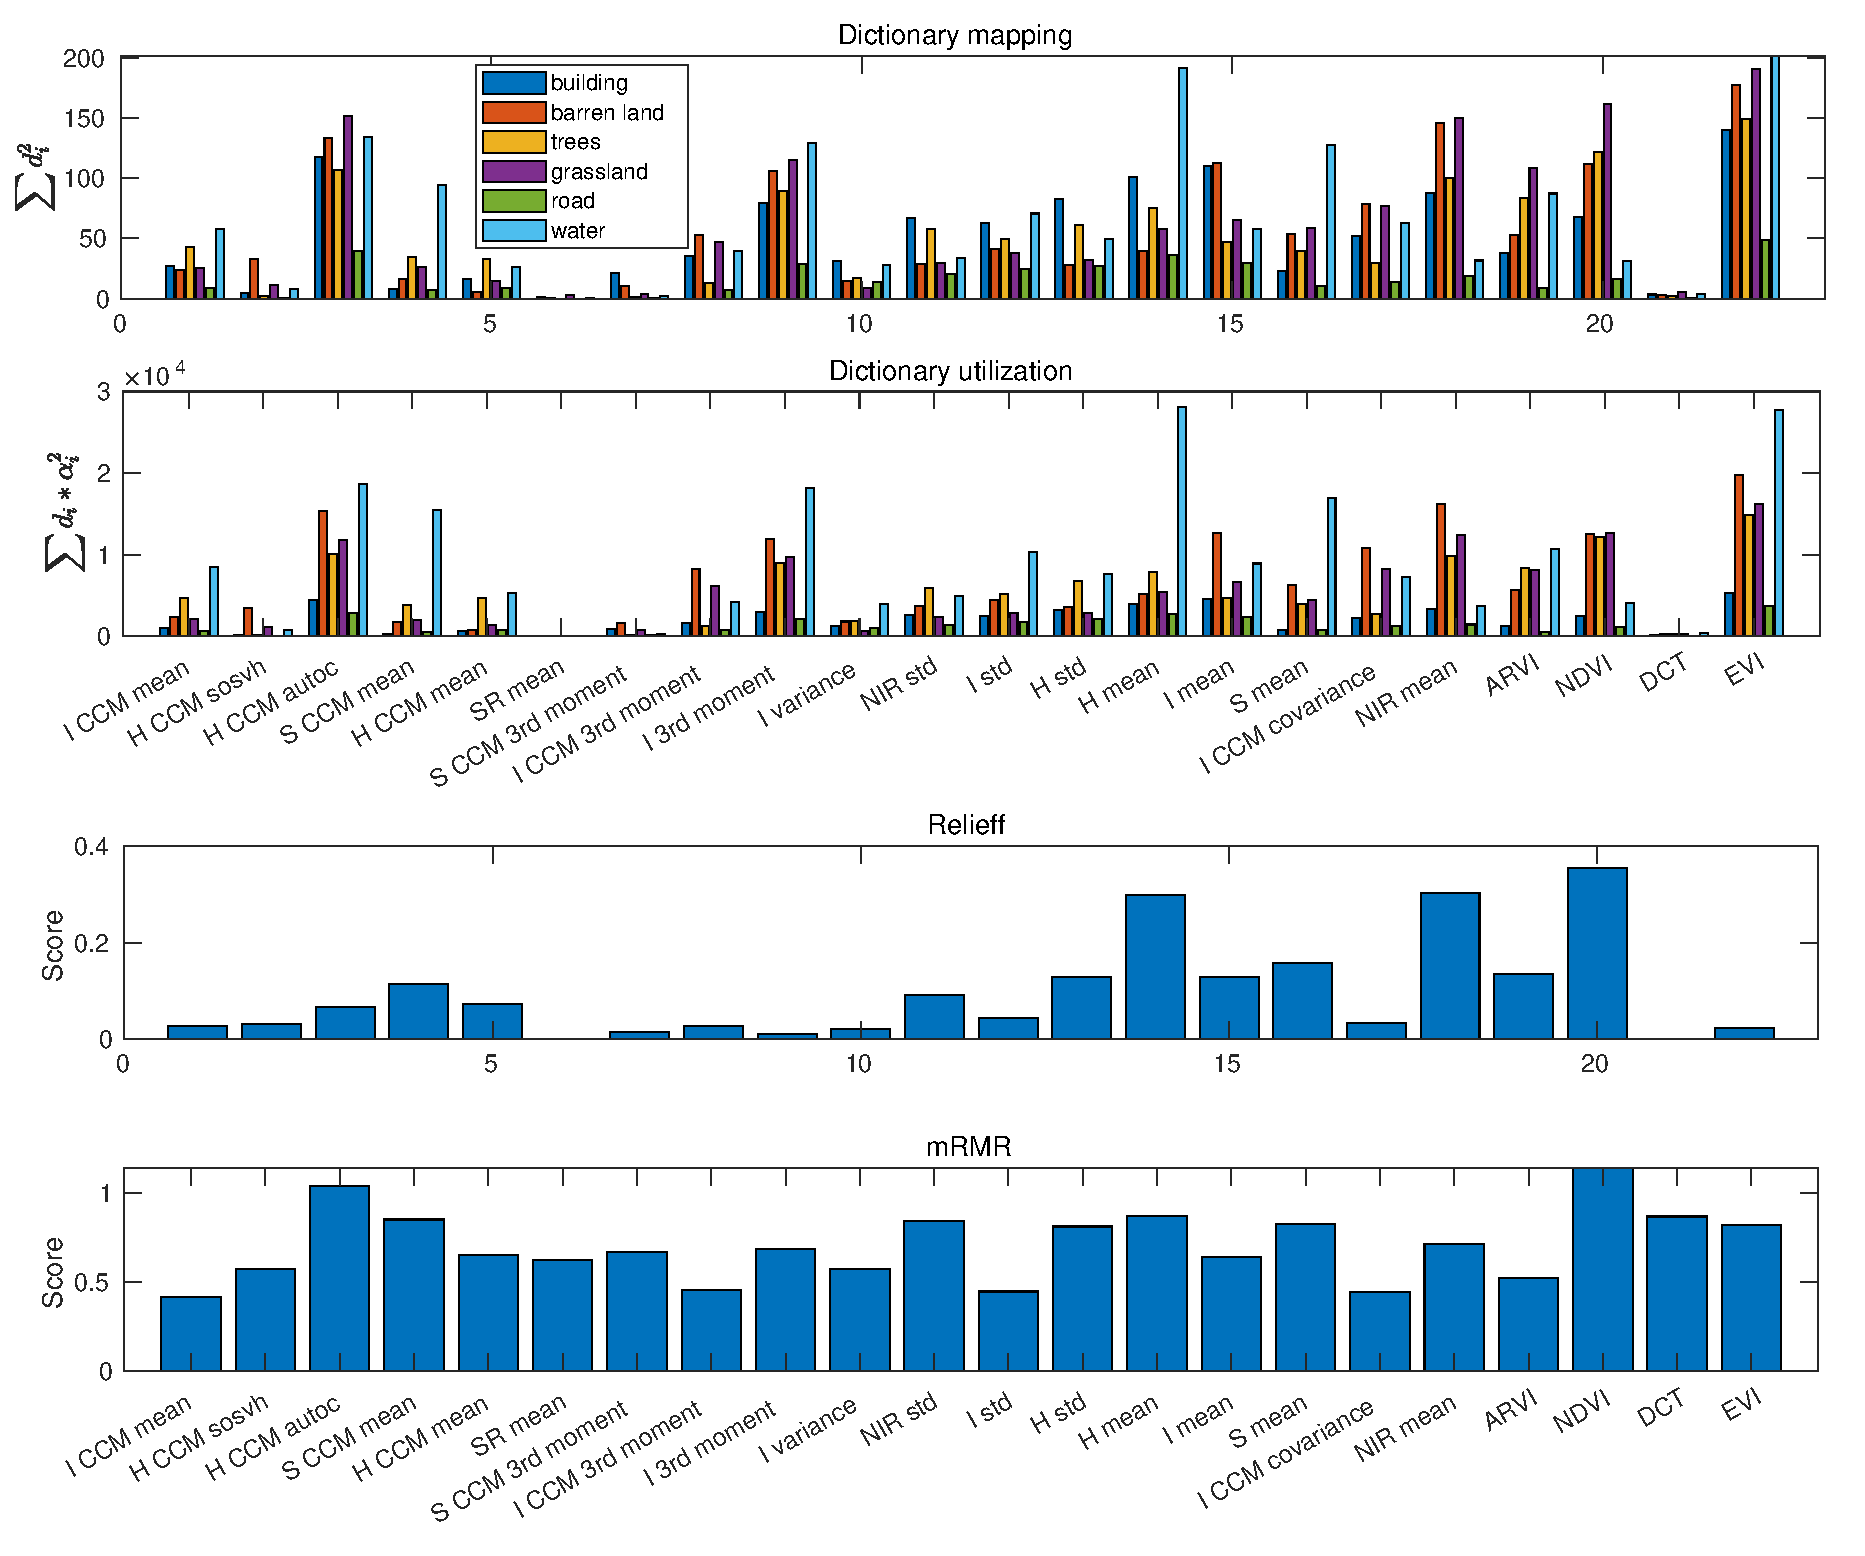
\includegraphics[width=5.7in]{Dict_FR.eps}
\caption{FR scores obtained using various methods on the Sat-6 dataset. The dictionary scores were obtained using frozen KSVD sparse representation.}%
\label{fig:FR}%
\end{figure*}


Authors in \cite{Basu2015} analyzed 150 total features using the Distribution Separability Criterion (DSC) and identified 22 prominent features. These features include the mean, standard deviation, $2^\textrm{nd}$ moment, and variance of Hue (H), Saturation (S), and Intensity (I). The color co-occurrence matrix (CCM, described in \cite{Boyda2017}) is calculated for each $H$, $S$, and $I$. Various statistics are calculated using each CCM, including the sum of squares for variance (SSOVH), auto-correlation (AUTOC), covariance, as well as the mean, standard deviation, $2^\textrm{nd}$ moment, and variance. Several established vegetation indices are used to differentiate vegetation. Which include Simple Ratio or Ratio Vegetation Index (SR or RVI) \cite{Jordan1969}, Atmospherically Resistant Vegetation Index (ARVI) \cite{Kaufman1992}, Normalized Vegetation Index (NDVI) \cite{Rouse1974}, and Enhanced Vegetation Index(EVI) \cite{Huete2002}. Finally, the Discrete Cosine Transformation (DCT) is calculated for the image.

Our work utilizes the same $22$ features as in \cite{Basu2015}, with some modifications. For a given image, we use the mean values of the vegetation indices. We use the second-highest frequency component position of the DCT, as this value contains the most discriminatory information. The feature vector obtained from each image, $F_i$, has a dimension of $22\times1$. This small dimension significantly reduces the computational workload of sparse coding and classification while maintaining high accuracy.

In addition to modifying some of the extracted features, another significant difference in our feature analysis involves the normalization process. The authors in \cite{Basu2015} normalized the features using the whole set of images (both training and testing). Since this would assume the availability of the testing images at the time of the model training, our work normalized the features using only the \textit{min} and \textit{max} values of the training set. Five percent buffer is set to the \textit{min} and \textit{max} values when normalizing to account for possible variability in the testing image features. When normalizing, the $2^\textrm{nd}$ moment and the variance become the same. Hence, the $3^\textrm{rd}$ moment is used instead of the $2^\textrm{nd}$ moment. The features are then converted to a logarithmic scale since we have observed that the data is more concentrated towards the origin. This leads to more distributed features and increased classification accuracy. The final list of features is listed in table \ref{table: Features}.

\subsection{Feature ranking}

The validity of the selected handcrafted features has to be evaluated using FR methods. Fig. \ref{fig:FR} shows the \textit{dictionary mapping} and the \textit{dictionary utilization} of the sparse coefficients used by dictionary elements projected into the original feature space from the frozen KSVD method on Sat-6 data. Since each dictionary atom is associated with a class, the class-wise metric analysis is performed on the original features. It also shows the FR done by the non-class specific Releiff and mRMR methods. Both proposed metrics perform similarly. While their scores are closer to the Relieff metric, they can capture some important features predicted by the mRMR method (e.g. \textit{H CCM autoc} and \textit{EVI}). The proposed metrics match with the Relieff metric in identifying SR mean and DCT as underutilized features.

The shortcomings of SR are well recorded in cases where an abundance of bare soil is present, and indices like Soil Adjusted Vegetation Indexes (SAVI) can be used to mitigate this problem \cite{Huete1988}. Presence of similar texture in both \textit{barren land} and \textit{grassland} classes, leads DCT component to have similar value. Since we have used a modified and more statistically condensed version of the 22 features selected by \cite{Basu2015}, some features do not perform well with the sparse model. Using sparse coding and linear classifiers, we can identify, evaluate, and improve the necessary input features that might increase the performance of the classification.

\section{Malware Detection by Analyzing CFGs of Binary Files}


In recent years the number of attacks by malware shared through the internet has increased. To avoid damage to the computer systems effective identification and classification of the malicious programs from the benign programs are necessary. There are several malware detection methods mainly categorized as static and dynamic \cite{Akhtar2021}. In dynamic detection, the suspicious program is activated in a sandbox or an emulator to observe the behavior. This would take a longer time, resources, and setup. Still, some suspicious activities might not be detected due to a lack of specific hardware or configurations. Static analysis just observes the source code of the suspicious program and tries to determine its validity. This method is much faster, however prone to ignoring run-time attacks. In this research, we will be focusing on the static analysis of binary files using control flow graphs (CFGs). We will narrow our focus on our research further by focusing only on portable executable (\textit{.exe}) files. It has not been established that there is a significant difference between CFGs belonging to malware and benign programs. Hence, we hypothesize that there is a significant difference between the graph structures of malware and benign programs.

This research is funded through the Department of Homeland Security (DHS) under the project \say{Cyber QR Ops: Improving the Quality and Resiliency of Critical Computing Infrastructure}. The research focus is to explore the viability of ML as an effective tool in identifying malware through graph analysis of CFGs. As the initial step, we would curate a dataset of benign and malicious programs with a publicly available dataset and malware dataset provided by \textit{Hoplite industries}.

The overview of the typical analysis is shown in figure \ref{fig: binary_ML}. First, the binary files are converted into CFGs. This is carried out by \textit{CFGFast()} function of the \textit{angr} python library \cite{shoshitaishvili2016state, stephens2016driller, shoshitaishvili2015firmalice }. Then the graphs are converted to a vector representation using \textit{Graph2Vec} algorithm\cite{Narayanan2017}. It can be seen that usually a dictionary of rooted sub-graphs is learned and then the similarity is calculated between the sub-graphs and the main graph representation. SR is a prime candidate for this operation due to its ability in learning dictionaries efficiently.

Typical implementations of the \textit{Graph2Vec} is shown in figure \ref{fig: G2V}, where the graphs are first converted into a word document using the Weisfeiler-Lehman graph kernel \cite{Shervashidze2011} and then uses \textit{Doc2Vec} \cite{Le2014}. We are proposing to replace the \textit{Doc2Vec} step with SR methods so better interpretability can be achieved between the classifier performance and the sub-graph features. Using our proposed FR metrics we are aiming to identify important sub-graph structures related to malware. 

\begin{figure*}[!t]%
\centering
\includegraphics[width=5.4in]{Figures/binary_ML_overview.png}
\caption{Overview of binary file analysis using CFGs}%
\label{fig: binary_ML}%
\end{figure*}

\begin{figure*}[!t]%
\centering
\includegraphics[width=5.4in]{Figures/G2V_overview.png}
\caption{Graph2Vec implementation overview with WL hash words and Word2Vec algorithms. We are proposing to replace the Word2Vec step with Sparse coding methods}%
\label{fig: G2V}%
\end{figure*}

\section{Expected outcomes and Broader Impacts}

\subsection{Research outcomes}

The main outcome will be the introduction of two well-defined FR metrics with mathematical and experiment validation. The introduced metrics will increase the utility of SR methods for a wide variety of datasets. A guide to conducting FR using examples from two ML domains will be presented with thorough details about setup and analysis. Discussion about relevant features in LULC applications will be conducted to identify necessities in each class. Discussion about SR compatibility in Malware detection will be explored. 

Some of the challenges will be the mathematical proof of optimal guarantee from the proposed metrics. We would hope to at least show the mathematical relationship to other common FR metrics measurements. Further, the experimental results with the different datasets would not conform to our expected performance. However, we would be able to establish the limitations of the proposed metrics. 

The proposed metrics are aimed to improve the fundamental workflow of the machine learning pipeline. Hence the outcomes of this proposal could improve the ML applications in a wide variety of domains. Hence The overall outcomes will have academic and societal benefits.     
\subsection{Academic benefits}

\begin{enumerate}
    \item Framework for the researchers to understand model behavior concerning the input feature.
    
    The ability to identify important/relevant features in an ML model gives insight into the training and learning process. Even for \say{black box} models having an input-output relationship allows to approximate the model behavior.
    
    \item Improving the ability to make smart choices of the number of features collected, stored, and processed.
    
    Often the most time-consuming part of research is the data collection and processing. If we could identify the most relevant features, the time spent on data collection can be efficiently used for other tasks.
    
    \item Reducing the computational, memory, time, and energy cost of ML models.
    
    With the increase in the number of features the dimensionality of the dataset increases. Which requires Larger storage facilities, high-end computational resources, fast transfer channels, longer wait periods, and higher energy costs. By using FR, we can identify the most relevant features to work with, saving limited resources.
\end{enumerate}

\subsection{Societal benefits}
The main societal benefactors of this proposal would be individuals and (small) business's who are interested in adapting ML for their operations.
\begin{enumerate}
    \item Demystify ML process through intuitive modeling.
    
    Most of the general public and businesses are excited about the ML methods. However, due to the \say{black box} nature of the models, they do not have an intuitive understanding of the model. For example, in an online movie streaming company the ML model is trained for the prediction of which customers are likely to cancel their subscription. But without an intuitive model, they cannot identify which features of the customer are contributing to the decision.  With an intuitive FR metric, the company can detect which features are mostly contributing. If the customers' watch time of romantic movies (feature)  is identified as the most significant factor, with the investigation it might be possible to understand if the platform has an issue with romantic movies. The company can add more romantic movies to the platform or suggest/market more romantic movies to retain the customer.
    
    \item Ability to assess the ML readiness of existing data.
    
    If a business is trying to adapt ML to its operations, it is better to assess the ML readiness of the business before investing money in ML. Let's say a shop wants to predict which customers are likely to return to their shop. They have collected some information (features) about the customers like time of the shopping, duration of the shopping, money spend, etc. With an intuitive FR method, it could be determined whether the data at hand is sufficient for effective ML training. If the collected features are not sufficient or highly correlated, The shop can collect different data for the ML process. 
    
    \item Publicly available source code.
    
    We are hoping to publish the code as an open-source so that interested parties can freely use the metrics. This will lead to wider usage of the proposed metrics and feedback on the effectiveness of the metrics in a wide variety of applications.

\end{enumerate}
\newpage
\bibliographystyle{ieeetr}
\bibliography{Bib_ENGR694.bib}

\newpage
\includepdf[pages=-, pagecommand={}]{NSF_BioSketch}

\end{document}
